\documentclass[12pt,a4paper]{article}

% =====================================================
% PACOTES
% =====================================================
\usepackage[utf8]{inputenc}
\usepackage[T1]{fontenc}
\usepackage[brazil]{babel}
\usepackage{geometry}
\usepackage{graphicx}
\usepackage{fancyhdr}
\usepackage{titlesec}
\usepackage{xcolor}
\usepackage{hyperref}
\usepackage{setspace}
\usepackage{enumitem}
\usepackage{newtxtext,newtxmath}
\usepackage[most]{tcolorbox}
\usepackage{qrcode}
\usepackage{float}
\usepackage{tikz}
\usepackage{colortbl}
\usetikzlibrary{arrows.meta, positioning}

\geometry{
    top=2.5cm,
    bottom=3cm,
    left=1.5cm,
    right=1.5cm
}

\onehalfspacing

% =====================================================
% CORES PERSONALIZADAS
% =====================================================
\definecolor{azulObjetivos}{RGB}{30,60,90}
\definecolor{cinzaCodigo}{RGB}{245,245,245}
\definecolor{vermelhoCodigo}{RGB}{180,50,50}
\definecolor{pretoTabela}{RGB}{0,0,0}
\definecolor{cinzaTabela}{RGB}{235,235,235}
\definecolor{mostarda}{RGB}{204,153,0}
\definecolor{azulTitulo}{RGB}{30,60,90}

% =====================================================
% BOX VISUALS
% =====================================================
\newtcolorbox{boxObjetivos}{
    colback=azulObjetivos!10,
    colframe=azulObjetivos,
    boxrule=1pt,
    arc=4pt,
    left=6pt,
    right=6pt,
    top=6pt,
    bottom=6pt,
    title=Objetivos
}

\newtcolorbox{boxCodigo}{
    breakable,
    colback=cinzaCodigo,
    colframe=vermelhoCodigo,
    boxrule=0.8pt,
    arc=2pt,
    left=6pt,
    right=6pt,
    top=6pt,
    bottom=6pt,
    borderline={0.5pt}{0pt}{vermelhoCodigo,dashed}
}

\newtcolorbox{boxAtividade}[1][]{
    breakable,
    enhanced,
    colback=azulTitulo!5,
    colframe=azulTitulo,
    boxrule=0pt,
    arc=6pt,
    outer arc=6pt,
    boxsep=0pt,
    left=14pt,
    right=14pt,
    top=16pt,
    bottom=14pt,
    title=#1,
    coltitle=white,
    colbacktitle=azulTitulo,
    fonttitle=\bfseries,
    attach boxed title to top left={
        yshift=-3mm,
        xshift=6mm
    },
    boxed title style={
        sharp corners,
        boxrule=0pt
    }
}

\newtcolorbox{boxDica}{
    colback=blue!5,
    colframe=azulTitulo,
    title=\textbf{Dicas Úteis},
    fonttitle=\bfseries,
    arc=2mm,
    boxrule=0.8pt
}

% =====================================================
% CABEÇALHO E RODAPÉ
% =====================================================
\pagestyle{fancy}
\fancyhf{}
\fancyhead[L]{
\includegraphics[height=1.8cm]{figures/garopaba_horizontal_marca2015_PNG.png}}
\fancyhead[R]{
\textbf{CST em Sistemas para Internet}\\
\textbf{UC: Programação para Internet 1}\\
Docente: Prof. André Moraes\\ 
IFSC -- Campus Garopaba
}
\fancyfoot[L]{\small\textit{\leftmark}}
\fancyfoot[R]{\small Página \thepage}
\renewcommand{\footrulewidth}{2.4pt}
\setlength{\headheight}{45pt}

% =====================================================
% ESTILO DE SEÇÃO
% =====================================================
\titleformat{\section}{\normalfont\Large\bfseries\color{azulTitulo}}{\thesection}{1em}{}[\vspace{0.3cm}\hrule]
\titleformat{\subsection}{\normalfont\bfseries}{}{0em}{}[\vspace{0.2cm}\hrule]

% =====================================================
% DOCUMENTO
% =====================================================
\begin{document}

\begin{center}
    {\Large \textbf{CADERNO DE ROTEIROS PRÁTICOS}}\\
    Unidade Curricular: Programação para Internet 1\\
    CST Sistemas para Internet -- Semestre 1
\end{center}

\vspace{0.5cm}
\hrule
\vspace{0.8cm}

\tableofcontents
\newpage

\section{Visão Geral da Unidade Curricular}

Esta unidade curricular foca no desenvolvimento de interfaces interativas e dinâmicas utilizando as tecnologias fundamentais da web. O cronograma está organizado em 8 roteiros progressivos:

\begin{enumerate}
    \item \textbf{Fundamentos da Web e Estrutura HTML5}
    \item \textbf{HTML5 Semântico e Estrutura de Mini-Sites}
    \item \textbf{Estilização com CSS3 e Box Model}
    \item \textbf{Layouts Modernos: Flexbox e Grid}
    \item \textbf{Responsividade e Frameworks CSS}
    \item \textbf{Lógica de Programação com JavaScript}
    \item \textbf{Roteiro Intermediário: Manipulação da Árvore DOM} \\
    Foco intensivo em métodos de seleção, criação e eventos.
    \item \textbf{Consumo de APIs e Requisições Assíncronas (Fetch)} \\
    Integração de dados externos (JSON) no frontend.
\end{enumerate}

\newpage

% ----------------------------------------------------------------------
% OMITINDO ROTEIROS 1-6 PARA FOCO NO DOM
% ----------------------------------------------------------------------

% =====================================================
% ROTEIRO PRÁTICO 01
% =====================================================

\section{Roteiro Prático 01 — Fundamentos da Web, HTML5 e Versionamento}

% =====================================================
% OBJETIVOS
% =====================================================

\begin{boxObjetivos}
\textbf{Objetivos da Aula}

Ao final desta aula o estudante será capaz de:

\begin{itemize}
\item Compreender a evolução da Internet e o papel do HTML;
\item Identificar os principais componentes de um documento HTML5;
\item Criar uma página web estruturada corretamente;
\item Utilizar tags básicas para organização de conteúdo;
\item Executar versionamento com Git e GitHub desde o início do projeto.
\end{itemize}
\end{boxObjetivos}

% =====================================================
% INTRODUÇÃO
% =====================================================

\subsection{Introdução}

A Internet transformou profundamente a forma como pessoas, empresas e governos produzem, compartilham e consomem informação. 

Sua origem remonta à década de 1960, com a ARPANET, projeto militar norte-americano que buscava criar uma rede descentralizada de comunicação entre computadores.

Na década de 1990, Tim Berners-Lee desenvolveu a World Wide Web (WWW), criando:

\begin{itemize}
\item O protocolo HTTP;
\item O conceito de URL;
\item A linguagem HTML;
\item O primeiro navegador web.
\end{itemize}

A Web evoluiu em diferentes fases:

\begin{itemize}
\item \textbf{Web 1.0}: páginas estáticas;
\item \textbf{Web 2.0}: interação e redes sociais;
\item \textbf{Web 3.0}: dados inteligentes e descentralização.
\end{itemize}

O HTML (HyperText Markup Language) é a base estrutural de praticamente toda aplicação web.

Mesmo sistemas complexos desenvolvidos em outras linguagens entregam HTML ao navegador.

% =====================================================
% PARTE 1
% =====================================================

\subsection{Parte 1 — Fundamentos da Internet}

\subsubsection{Como funciona uma página web?}

Quando um usuário digita uma URL no navegador:

\begin{enumerate}
\item O navegador envia uma requisição HTTP;
\item O servidor responde enviando um documento HTML;
\item O navegador interpreta o HTML;
\item O conteúdo é renderizado na tela.
\end{enumerate}


\begin{boxAtividade}[Atividade Prática 1 - Pesquisa dirigida]

Pesquise e escreva uma definição objetiva (máx. 4 linhas cada) para:

\begin{itemize}
\item ARPANET
\item Tim Berners-Lee
\item W3C
\item HTTP
\item URL
\item Navegador Mosaic
\item Web 1.0, 2.0 e 3.0
\end{itemize}

Em seguida, responda:

\textit{Qual foi o principal impacto da Web na transformação da sociedade digital?}

\end{boxAtividade}




% =====================================================
% PARTE 2
% =====================================================

\subsection{Parte 2 — Estrutura Base do Documento HTML5}

\subsubsection{Estrutura mínima obrigatória}

\begin{boxCodigo}
\begin{verbatim}
<!DOCTYPE html>
<html lang="pt-BR">
<head>
    <meta charset="UTF-8">
    <title>Prog. Internet I - 2026</title>
</head>
<body>

</body>
</html>
\end{verbatim}
\end{boxCodigo}



\begin{boxAtividade}[Atividade prática 2 — Criando o Projeto]

\begin{itemize}
\item Criar diretório \texttt{prog-internet-2026};
\item Criar arquivo \texttt{index.html};
\item Inserir a estrutura base HTML5;
\item Testar no navegador.
\end{itemize}

\end{boxAtividade}

\vspace{0.5cm}

\begin{boxAtividade}[Micro-Commit 1 — Estrutura Inicial]

\begin{boxCodigo}
\begin{verbatim}
git init
git add .
git commit -m "Estrutura inicial HTML5"
\end{verbatim}
\end{boxCodigo}

\end{boxAtividade}


% =====================================================
% PARTE 3
% =====================================================

\subsection{Parte 3 — Comandos Básicos HTML5}

\begin{boxTabela}
\rowcolors{2}{cinzaTabela!40}{white}
\begin{tabular}{|p{3cm}|p{13cm}|}
\hline
\rowcolor{pretoTabela}
\color{white}\textbf{TAG} & 
\color{white}\textbf{Definição} \\
\hline
<!DOCTYPE html> & Define documento HTML5 \\
<html> & Estrutura geral da página \\
<head> & Informações da página \\
<meta charset="UTF-8"> & Codificação \\
<title> & Título da aba \\
<body> & Conteúdo visível \\
<h1> até <h6> & Títulos \\
<p> & Parágrafo \\
<hr> & Linha horizontal \\
<ul> / <li> & Lista não ordenada \\
<pre> & Texto pré-formatado \\
<a> & Hiperlink \\
\hline
\end{tabular}
\end{boxTabela}

\begin{boxAtividade}[Atividade 3 — Inserindo Conteúdo]

Adicionar ao \texttt{<body>}:

\begin{itemize}
\item Título da disciplina;
\item Subtítulo com seu nome;
\item Parágrafo explicando o que você entende por Internet;
\item Lista com 3 tecnologias que deseja aprender;
\item Duas linhas horizontais (\texttt{<hr>});
\item Bloco \texttt{<pre>} contendo:
    \begin{itemize}
        \item Seu curso;
        \item Seu semestre;
        \item Data atual.
    \end{itemize}
\end{itemize}

Após implementar, teste novamente no navegador.

\end{boxAtividade}

\vspace{0.5cm}

\begin{boxAtividade}[Micro-Commit 2 — Conteúdo Estruturado]

Registre a evolução do projeto:

\begin{boxCodigo}
\begin{verbatim}
git add .
git commit -m "Adicionando conteúdo estruturado"
\end{verbatim}
\end{boxCodigo}

\end{boxAtividade}

\newpage
% =====================================================
% PARTE 4
% =====================================================

\subsection{Parte 4 — Trabalhando com Links}

\subsubsection{Exemplo}

\begin{boxCodigo}
\begin{verbatim}
<a href="https://www.ifsc.edu.br" target="_blank">
    Página do IFSC
</a>
\end{verbatim}
\end{boxCodigo}




\begin{boxAtividade}[Atividade 4 — Trabalhando com Links e Comentários]

Adicionar ao final da página:

\begin{itemize}
\item Um link para o site do IFSC;
\item Um link para o site do W3C;
\item Um comentário HTML explicando qual foi sua maior dificuldade na atividade.
\end{itemize}

Os links devem abrir em nova aba utilizando o atributo \texttt{target="\_blank"}.

Após implementar, teste novamente no navegador.

\end{boxAtividade}

\vspace{0.5cm}

\begin{boxAtividade}[Micro-Commit 3 — Links e Comentários]

Registre a evolução do projeto:

\begin{boxCodigo}
\begin{verbatim}
git add .
git commit -m "Adicionando links externos e comentário HTML"
\end{verbatim}
\end{boxCodigo}

\end{boxAtividade}



\newpage
% =====================================================
% PARTE 5
% =====================================================

\subsection{Parte 5 — Versionamento com Git e GitHub}

\begin{boxAtividade}[Atividade 5 — Publicando o Projeto no GitHub]

\textbf{Passo 1 — Criar repositório no GitHub}

\begin{itemize}
\item Acesse: \texttt{https://github.com}
\item Clique em \textbf{New Repository}
\item Nomeie como: \texttt{prog-internet-2026}
\item Selecione como \textbf{Public}
\item NÃO marque a opção para criar README automaticamente
\item Clique em \textbf{Create repository}
\end{itemize}

\vspace{0.5cm}

\textbf{Passo 2 — Executar comandos no terminal}

No diretório do seu projeto, execute:

\begin{boxCodigo}
\begin{verbatim}
echo "# prog-internet-2026" >> README.md
git init
git add README.md
git add .
git commit -m "Primeiro commit - Estrutura inicial"
git branch -M main
git remote add origin https://github.com/SEU-USUARIO/prog-internet-2026.git
git push -u origin main
\end{verbatim}
\end{boxCodigo}

Se solicitado, utilize seu usuário e token de autenticação do GitHub.

\vspace{0.5cm}

\textbf{Resultado Esperado}

\begin{itemize}
\item O arquivo \texttt{index.html} deve estar visível no repositório;
\item O arquivo \texttt{README.md} deve estar criado;
\item O repositório deve conter pelo menos um commit inicial.
\end{itemize}

\end{boxAtividade}

\vspace{0.5cm}

\begin{boxAtividade}[Boas Práticas a partir desta Aula]

\begin{itemize}
\item Todo código desenvolvido será versionado;
\item Cada etapa significativa deverá gerar um commit;
\item O histórico de commits fará parte da avaliação formativa;
\item Organização e clareza no repositório são critérios avaliativos.
\end{itemize}

\end{boxAtividade}
% =====================================================
% CHECKLIST
% =====================================================

\subsection{Checklist Final de Verificação}

\begin{boxAtividade}[Checklist Técnico]

Antes de finalizar o roteiro, verifique:

\begin{itemize}
\item O documento inicia com \texttt{<!DOCTYPE html>};
\item A tag \texttt{<html>} contém o atributo \texttt{lang="pt-BR"};
\item O \texttt{<meta charset="UTF-8">} está corretamente definido;
\item O código está indentado e organizado;
\item Os links utilizam \texttt{target="\_blank"};
\item O repositório contém pelo menos três commits distintos;
\item O arquivo está corretamente publicado no GitHub.
\end{itemize}

\end{boxAtividade}

\vspace{0.5cm}

\begin{boxAtividade}[Observação Técnica Importante]

A tag \texttt{<font>} foi descontinuada no HTML5.

Toda formatação visual deve ser realizada utilizando CSS, que será introduzido nos próximos roteiros.

\end{boxAtividade}

\newpage




% =====================================================
% ROTEIRO PRÁTICO 02
% =====================================================

\section{Roteiro Prático 02 — HTML5 Semântico, CSS Externo e Estrutura Profissional}

% =====================================================
% OBJETIVOS
% =====================================================

\begin{boxObjetivos}
\textbf{Objetivos da Aula}

Ao final desta aula o estudante será capaz de:

\begin{itemize}
\item Utilizar corretamente HTML5 semântico;
\item Organizar múltiplas páginas interligadas;
\item Criar e conectar um arquivo CSS externo;
\item Trabalhar com imagens utilizando caminhos relativos;
\item Estruturar diretórios de forma profissional;
\item Aplicar versionamento incremental com Git.
\end{itemize}
\end{boxObjetivos}

% =====================================================
% INTRODUÇÃO
% =====================================================

\subsection{Introdução}

No roteiro anterior construímos uma página HTML básica e iniciamos o versionamento com Git.

Agora avançaremos para um modelo mais próximo de aplicações reais, organizando um mini-site com múltiplas páginas, estrutura semântica adequada e separação entre conteúdo (HTML) e estilo (CSS).

A separação entre estrutura e apresentação é um dos pilares do desenvolvimento web moderno. O HTML é responsável pela organização do conteúdo, enquanto o CSS define a aparência visual da aplicação.

Neste roteiro construiremos um mini-site institucional com organização profissional.

% =====================================================
% FUNDAMENTAÇÃO TEÓRICA
% =====================================================

\subsection{Fundamentação Teórica — HTML5 Semântico}

O HTML5 introduziu uma abordagem mais semântica para organização de páginas web.  
Isso significa que as tags passaram a descrever o significado estrutural do conteúdo.

A semântica melhora:

\begin{itemize}
\item Organização do código;
\item Acessibilidade;
\item SEO (Search Engine Optimization);
\item Manutenção e escalabilidade do projeto.
\end{itemize}

\subsection{Principais Tags Estruturais do HTML5}

\begin{boxTabela}
\rowcolors{2}{cinzaTabela!20}{white}
\begin{tabular}{|p{3.5cm}|p{12.5cm}|}
\hline
\rowcolor{pretoTabela}
\color{white}\textbf{Tag} &
\color{white}\textbf{Função Estrutural} \\
\hline

<header> & Cabeçalho da página ou seção. \\
\hline
<nav> & Área de navegação principal. \\
\hline
<main> & Conteúdo principal da página. \\
\hline
<section> & Agrupamento temático de conteúdo. \\
\hline
<article> & Conteúdo independente (post, card, notícia). \\
\hline
<aside> & Conteúdo complementar ou lateral. \\
\hline
<footer> & Rodapé da página ou seção. \\
\hline
<link> & Conexão com arquivos externos (CSS). \\
\hline
<img> & Inserção de imagem (com atributo alt obrigatório). \\
\hline
\end{tabular}
\end{boxTabela}

\subsection{Boas Práticas}

Evite estruturar páginas apenas com <div>.  
Utilize as tags semânticas para tornar o código mais claro e profissional.



\begin{boxDica}

\textbf{Atalhos Importantes no VS Code para HTML}

    \begin{itemize}
    \item Digite \texttt{!} e pressione \texttt{TAB} para gerar automaticamente a estrutura básica do HTML5.
    \item Para formatar automaticamente o código: 
    \begin{itemize}
        \item \texttt{OPTION + SHIFT + I} [Mac].
        \item \texttt{ALT + SHIFT + I} [Linux].
        \item \texttt{ALT + SHIFT + F} [Windows].
    \end{itemize}
    \item Utilize \texttt{CTRL + /} para comentar ou descomentar linhas.
    \item Use \texttt{CTRL + Espaço} para ativar sugestões automáticas.
    \item Utilize \texttt{CTRL + S} frequentemente para salvar alterações.
    \end{itemize}
    
    \textbf{Dica Profissional:}  
    Acostume-se a trabalhar com código bem indentado e organizado desde o início. Isso faz parte da avaliação formativa.

\end{boxDica}



% =====================================================
% SEQUÊNCIA RECOMENDADA DE USO
% =====================================================

\begin{boxDica}

\textbf{Sequência Recomendada de Uso do Git}

Sempre que finalizar uma etapa do trabalho, utilize a seguinte sequência:

\begin{boxCodigo}
\begin{verbatim}
git status
git add .
git commit -m "Descrição clara da alteração"
git push
\end{verbatim}
\end{boxCodigo}

\textbf{Boa prática:}
\begin{itemize}
\item Faça commits pequenos e frequentes;
\item Utilize mensagens descritivas;
\item Evite acumular muitas alterações em um único commit.
\end{itemize}

\end{boxDica}



\newpage
% =====================================================
% PARTE 1 — ESTRUTURA DO PROJETO
% =====================================================

\subsection{Parte 1 — Organização Profissional do Projeto}

Estrutura recomendada:

\begin{boxCodigo}
\begin{verbatim}
prog-internet-2026/
│
└── roteiro02/
    ├── index.html
    ├── sobre.html
    ├── contato.html
    └── assets/
        ├── css/
        │   └── style.css
        └── img/
            └── perfil.jpg
\end{verbatim}
\end{boxCodigo}

\begin{boxAtividade}[Atividade 1 — Criando Estrutura Base]

\begin{itemize}
\item Criar pasta \texttt{roteiro02};
\item Criar os três arquivos HTML;
\item Criar pasta \texttt{assets/css};
\item Criar pasta \texttt{assets/img};
\item Criar arquivo \texttt{style.css}.
\end{itemize}

\end{boxAtividade}

\begin{boxAtividade}[Micro-Commit 1]

\begin{boxCodigo}
\begin{verbatim}
git add .
git commit -m "Criando estrutura profissional roteiro 02"
\end{verbatim}
\end{boxCodigo}

\end{boxAtividade}

% =====================================================
% PARTE 2 — ESTRUTURA SEMÂNTICA
% =====================================================

\subsection{Parte 2 — Estrutura HTML Semântica}
No arquivo \texttt{index.html}:

\begin{boxCodigo}
\begin{verbatim}
<!DOCTYPE html>
<html lang="pt-BR">
<head>
    <meta charset="UTF-8">
    <title>Mini-Site</title>
    <link rel="stylesheet" href="assets/css/style.css">
</head>
<body>

<header>
    <h1>Meu Mini-Site</h1>
</header>

<nav>
    <ul>
        <li><a href="index.html">Home</a></li>
        <li><a href="sobre.html">Sobre</a></li>
        <li><a href="contato.html">Contato</a></li>
    </ul>
</nav>

<main>
    <section>
        <h2>Conteúdo Principal</h2>
        <p>Texto da seção.</p>
    </section>
</main>

<footer>
    <p>Seu nome - 2026</p>
</footer>

</body>
</html>
\end{verbatim}
\end{boxCodigo}

\begin{boxAtividade}[Atividade 2 — Implementando Estrutura]

\begin{itemize}
\item Implementar estrutura nas três páginas;
\item Garantir navegação funcional;
\item Testar todos os links.
\end{itemize}

\end{boxAtividade}

\begin{boxAtividade}[Micro-Commit 2]

\begin{boxCodigo}
\begin{verbatim}
git add .
git commit -m "Implementando estrutura semantica completa"
\end{verbatim}
\end{boxCodigo}

\end{boxAtividade}

% =====================================================
% PARTE 3 — CSS EXTERNO
% =====================================================

\subsection{Parte 3 — Introdução ao CSS Externo}

No arquivo \texttt{style.css}:

\begin{boxCodigo}
\begin{verbatim}
body {
    font-family: Arial, sans-serif;
    margin: 0;
}

header {
    background-color: #003366;
    color: white;
    padding: 15px;
}

nav ul {
    list-style: none;
}

nav li {
    display: inline;
    margin-right: 15px;
}

footer {
    margin-top: 20px;
    font-size: 14px;
}
\end{verbatim}
\end{boxCodigo}

\begin{boxAtividade}[Atividade 3 — Aplicando CSS]

\begin{itemize}
\item Criar e conectar arquivo CSS;
\item Verificar funcionamento nas três páginas;
\item Ajustar estilos conforme necessário.
\end{itemize}

\end{boxAtividade}

\begin{boxAtividade}[Micro-Commit 3]

\begin{boxCodigo}
\begin{verbatim}
git add .
git commit -m "Adicionando estilo CSS externo"
\end{verbatim}
\end{boxCodigo}

\end{boxAtividade}

% =====================================================
% PARTE 4 — IMAGENS
% =====================================================

\subsection{Parte 4 — Inserindo Imagens}
No arquivo \texttt{index.html}:

\begin{boxCodigo}
\begin{verbatim}
<img src="assets/img/perfil.jpg" alt="Foto de perfil">
\end{verbatim}
\end{boxCodigo}

\begin{boxAtividade}[Atividade 4 — Trabalhando com Imagem]

\begin{itemize}
\item Inserir imagem na página inicial;
\item Utilizar atributo alt;
\item Garantir caminho relativo correto.
\end{itemize}

\end{boxAtividade}

\begin{boxAtividade}[Micro-Commit 4]

\begin{boxCodigo}
\begin{verbatim}
git add .
git commit -m "Adicionando imagem ao mini-site"
\end{verbatim}
\end{boxCodigo}

\end{boxAtividade}

% =====================================================
% CHECKLIST FINAL
% =====================================================

\subsection{Checklist Final}

\begin{boxAtividade}[Verificação Estrutural]

\begin{itemize}
\item Estrutura de diretórios organizada;
\item HTML semântico implementado corretamente;
\item CSS externo funcionando;
\item Navegação funcional;
\item Imagem carregando corretamente;
\item Pelo menos 4 commits realizados.
\end{itemize}

\end{boxAtividade}



% =====================================================
% PUBLICAÇÃO FINAL NO GITHUB
% =====================================================

\begin{boxAtividade}[Publicação Final no GitHub]

Após revisar o checklist:

\begin{itemize}
\item Verifique se todos os arquivos estão salvos;
\item Execute a sequência completa de versionamento;
\item Certifique-se de que o repositório remoto está atualizado.
\end{itemize}

\begin{boxCodigo}
\begin{verbatim}
git status
git add .
git commit -m "Finalizacao roteiro 02"
git push
\end{verbatim}
\end{boxCodigo}

\textbf{Resultado esperado:}

Todos os arquivos do roteiro02 devem estar visíveis no GitHub.

\end{boxAtividade}




% =====================================================
% ENTREGA DA ATIVIDADE
% =====================================================
\subsection{Entrega da atividade}
\begin{boxAtividade}[Entrega da Atividade]

Para concluir esta atividade, o estudante deverá:

\begin{itemize}
\item Confirmar que o repositório está atualizado no GitHub;
\item Copiar o link público do repositório;
\item Enviar apenas o link na tarefa correspondente no SIGAA.
\end{itemize}

\textbf{Exemplo de link esperado:}

\texttt{https://github.com/seu-usuario/prog-internet-2026}

\textbf{Importante:}
\begin{itemize}
\item O repositório deve estar público;
\item O histórico de commits será considerado na avaliação;
\item Não será necessário enviar arquivos compactados (.zip).
\end{itemize}

\end{boxAtividade}



\newpage
% =====================================================
% FUNDAMENTAÇÃO COMPLEMENTAR — PROPRIEDADES CSS
% =====================================================

\subsection{Fundamentação Complementar — Propriedades CSS Essenciais}

O CSS (Cascading Style Sheets) é responsável pela apresentação visual da página.  
Ele permite definir cores, espaçamentos, fontes, posicionamento e organização visual.

\subsection{Principais Propriedades CSS}

\begin{boxTabela}
\rowcolors{2}{cinzaTabela!20}{white}
\begin{tabular}{|p{4cm}|p{12cm}|}
\hline
\rowcolor{pretoTabela}
\color{white}\textbf{Propriedade} &
\color{white}\textbf{Função} \\
\hline

color & Define a cor do texto. \\
\hline

background-color & Define a cor de fundo do elemento. \\
\hline

font-family & Define a família da fonte. \\
\hline

font-size & Define o tamanho da fonte. \\
\hline

margin & Define o espaçamento externo do elemento. \\
\hline

padding & Define o espaçamento interno do elemento. \\
\hline

border & Define bordas ao redor do elemento. \\
\hline

width / height & Define largura e altura do elemento. \\
\hline

display & Define o tipo de exibição (block, inline, inline-block). \\
\hline

text-align & Define alinhamento do texto. \\
\hline

\end{tabular}
\end{boxTabela}

\subsection*{Exemplo Prático}

\begin{boxCodigo}
\begin{verbatim}
section {
    background-color: #f4f4f4;
    padding: 20px;
    margin: 10px;
}
\end{verbatim}
\end{boxCodigo}


\newpage
% =====================================================
% DICAS ESSENCIAIS — GIT E GITHUB
% =====================================================

\subsection{Dicas Essenciais — Git e GitHub}

O Git é a ferramenta de controle de versão utilizada nesta disciplina.  
Abaixo estão os principais comandos que você utilizará com frequência.

\begin{boxTabela}
\rowcolors{2}{cinzaTabela!20}{white}
\begin{tabular}{|p{4cm}|p{12cm}|}
\hline
\rowcolor{pretoTabela}
\color{white}\textbf{Comando} &
\color{white}\textbf{Função} \\
\hline

git status &
Mostra o estado atual do repositório (arquivos modificados, adicionados ou pendentes de commit). \\
\hline

git add . &
Adiciona todos os arquivos modificados para a área de preparação (staging area). \\
\hline

git commit -m "mensagem" &
Cria um novo commit com uma descrição clara da alteração realizada. \\
\hline

git push &
Envia os commits locais para o repositório remoto no GitHub. \\
\hline

git pull &
Atualiza seu repositório local com alterações feitas no repositório remoto. \\
\hline

\end{tabular}
\end{boxTabela}



\newpage





% =====================================================



% =====================================================
% ROTEIRO PRÁTICO 03
% =====================================================

\section{Roteiro Prático 03 — Publicação com GitHub Pages e Aprimoramento Visual}

    % =====================================================
    % OBJETIVOS
    % =====================================================
    
    \begin{boxObjetivos}
    \textbf{Objetivos da Aula}
    
    Ao final desta aula o estudante será capaz de:
    
    \begin{itemize}
    \item Refinar a estrutura visual do mini-site;
    \item Organizar o layout utilizando container centralizado;
    \item Aplicar efeitos visuais simples com CSS;
    \item Configurar e publicar o site utilizando GitHub Pages;
    \item Disponibilizar um link público funcional.
    \end{itemize}
    \end{boxObjetivos}

% =====================================================
% INTRODUÇÃO
% =====================================================
    
    \subsection*{Introdução}
    
    Até este momento construímos um mini-site estruturado com HTML5 semântico e CSS externo.
    
    Agora daremos um passo importante: tornar o projeto visualmente mais organizado e publicá-lo na internet utilizando o GitHub Pages.
    
    A publicação de um site estático permite que qualquer pessoa acesse sua aplicação por meio de um endereço público.
    
    Este é o primeiro contato com deploy web na disciplina.
    
    % =====================================================
    % PARTE 1 — MELHORANDO A ESTRUTURA
    % =====================================================
    
    \subsection{Parte 1 — Ajustes Estruturais}
    
    Adicionar dentro do <head> de todas as páginas:
    
    \begin{boxCodigo}
    \begin{verbatim}
    <meta name="viewport" content="width=device-width, initial-scale=1.0">
    \end{verbatim}
    \end{boxCodigo}
    
    Isso prepara o site para futura responsividade.

    % =====================================================
    % PARTE 2 — APRIMORANDO O CSS
    % =====================================================
    
    \subsection{Parte 2 — Aprimoramento Visual com CSS}
    
        Atualize o arquivo \texttt{style.css} com:
        
        \begin{boxCodigo}
        \begin{verbatim}
        body {
            font-family: Arial, sans-serif;
            margin: 0;
            background-color: #f2f2f2;
        }
        
        .container {
            width: 80%;
            margin: 0 auto;
        }
        
        header {
            background-color: #003366;
            color: white;
            padding: 20px;
            text-align: center;
        }
        
        nav ul {
            list-style: none;
            padding: 0;
            text-align: center;
        }
        
        nav li {
            display: inline;
            margin: 0 15px;
        }
        
        nav a {
            text-decoration: none;
            color: #003366;
            font-weight: bold;
        }
        
        nav a:hover {
            color: #ff6600;
        }
        
        section {
            background-color: white;
            padding: 20px;
            margin-top: 20px;
            border-radius: 8px;
            box-shadow: 0px 2px 6px rgba(0,0,0,0.1);
        }
        
        footer {
            margin-top: 30px;
            padding: 15px;
            text-align: center;
            font-size: 14px;
        }
        \end{verbatim}
        \end{boxCodigo}
        
        \begin{boxAtividade}[Atividade 1 — Aplicando Container]
        
        \begin{itemize}
        \item Envolver o conteúdo principal dentro de uma <div class="container">;
        \item Testar o alinhamento centralizado;
        \item Verificar se todas as páginas mantêm consistência visual.
        \end{itemize}
        
        \end{boxAtividade}
        
        \begin{boxAtividade}[Micro-Commit 1]
        
        \begin{boxCodigo}
        \begin{verbatim}
        git add .
        git commit -m "Aprimorando layout com container e efeitos visuais"
        \end{verbatim}
        \end{boxCodigo}
        
        \end{boxAtividade}
        
        % =====================================================
        % PARTE 3 — PUBLICANDO COM GITHUB PAGES
        % =====================================================
            
    \subsection{Parte 3 — Publicação com GitHub Pages}
        \subsubsection{Passo 1 — Atualizar repositório}
        
        \begin{boxCodigo}
        \begin{verbatim}
        git status
        git add .
        git commit -m "Preparando publicacao no GitHub Pages"
        git push
        \end{verbatim}
        \end{boxCodigo}
        
        \subsubsection{Passo 2 — Ativar GitHub Pages}
        
        No repositório no GitHub:
        
        \begin{itemize}
        \item Acessar \textbf{Settings};
        \item Clicar em \textbf{Pages};
        \item Em Source, selecionar:
            \begin{itemize}
                \item Branch: main
                \item Folder: /root
            \end{itemize}
        \item Salvar.
        \end{itemize}
        
        O GitHub fornecerá um endereço público no formato:
        
        \texttt{https://seu-usuario.github.io/prog-internet-2026/}
        
        % =====================================================
        % PARTE 4 — TESTANDO A PUBLICAÇÃO
        % =====================================================
        
        \subsubsection{Parte 4 — Verificação da Publicação}
            
            \begin{boxAtividade}[Atividade 2 — Teste de Acesso Público]
            
            \begin{itemize}
            \item Acessar o link fornecido pelo GitHub;
            \item Navegar entre as páginas;
            \item Verificar funcionamento da navegação;
            \item Testar em outro navegador ou dispositivo.
            \end{itemize}
            
            \end{boxAtividade}
        
% =====================================================
% CHECKLIST FINAL
% =====================================================


\subsection{Checklist Final}

    \begin{boxAtividade}[Verificação Geral]
    
    \begin{itemize}
    \item Layout centralizado;
    \item CSS aplicado corretamente;
    \item Efeito hover funcionando;
    \item Navegação funcional;
    \item GitHub Pages ativo;
    \item Site acessível por URL pública.
    \end{itemize}
    
    \end{boxAtividade}
    
    % =====================================================
    % ENTREGA
    % =====================================================
    
    \begin{boxAtividade}[Entrega da Atividade]
    
    O estudante deverá enviar no SIGAA:
    
    \begin{itemize}
    \item Link público do GitHub Pages;
    \item Link do repositório no GitHub.
    \end{itemize}
    
    Não é necessário enviar arquivos compactados.
    
    \end{boxAtividade}




    
\section*{6. FAQ – Problemas Comuns com Git e GitHub}
% =====================================================

Durante as atividades práticas com Git e GitHub, alguns erros podem ocorrer, principalmente em ambientes de laboratório Linux. Abaixo estão os problemas mais comuns e como resolvê-los rapidamente.

\subsection*{6.1 Erro: Please tell me who you are}

\textbf{Mensagem típica:}

\begin{verbatim}
*** Please tell me who you are.
Run
  git config --global user.email "you@example.com"
  git config --global user.name "Your Name"
\end{verbatim}

\textbf{Causa:}  
O Git precisa identificar quem está realizando o commit. Nome e e-mail ainda não foram configurados na máquina.

\textbf{Solução:}

Execute no terminal:

\begin{verbatim}
git config --global user.name "Seu Nome Completo"
git config --global user.email "seu_email@exemplo.com"
\end{verbatim}

Exemplo:

\begin{verbatim}
git config --global user.name "Maria da Silva"
git config --global user.email "maria@email.com"
\end{verbatim}

Após isso, tente novamente:

\begin{verbatim}
git commit -m "Mensagem do commit"
\end{verbatim}

\textbf{Observação:}  
Se o computador for compartilhado, pode-se configurar apenas para o repositório atual:

\begin{verbatim}
git config user.name "Seu Nome"
git config user.email "seu_email@exemplo.com"
\end{verbatim}

---

\subsection*{6.2 Erro: "fatal: unable to auto-detect email address"}

\textbf{Causa:}  
Mesmo problema do item anterior: o Git não tem nome e e-mail configurados.

\textbf{Solução:}  
Configurar o usuário conforme indicado na seção 6.1.

---

\subsection*{6.3 Erro ao dar push – senha não aceita}

\textbf{Mensagem típica:}

\begin{verbatim}
remote: Support for password authentication was removed
fatal: Authentication failed
\end{verbatim}

\textbf{Causa:}  
O GitHub não permite mais autenticação usando apenas senha.

\textbf{Soluções possíveis:}

\textbf{Opção 1 – Utilizar Token de Acesso (PAT):}
\begin{itemize}
    \item Gerar um token no GitHub.
    \item Usar o token no lugar da senha ao executar o \texttt{git push}.
\end{itemize}

\textbf{Opção 2 – Configurar autenticação via SSH:}
\begin{itemize}
    \item Gerar chave SSH com:
\begin{verbatim}
ssh-keygen -t ed25519 -C "seu_email@exemplo.com"
\end{verbatim}
    \item Adicionar a chave pública nas configurações do GitHub.
\end{itemize}

---

\subsection*{6.4 Verificar configurações atuais do Git}

Para conferir se o nome e e-mail estão configurados:

\begin{verbatim}
git config --list
\end{verbatim}

Ou apenas as configurações globais:

\begin{verbatim}
git config --global --list
\end{verbatim}

---

\subsection*{6.5 Erro: "nothing to commit"}

\textbf{Mensagem típica:}

\begin{verbatim}
nothing to commit, working tree clean
\end{verbatim}

\textbf{Causa:}  
Nenhuma alteração foi adicionada à área de stage.

\textbf{Solução:}

Verificar o status:

\begin{verbatim}
git status
\end{verbatim}

Adicionar arquivos:

\begin{verbatim}
git add nome_do_arquivo
\end{verbatim}

Ou todos os arquivos:

\begin{verbatim}
git add .
\end{verbatim}

Depois realizar o commit novamente.

---

\subsection*{6.6 Dica Importante}

Sempre que ocorrer um erro:
\begin{itemize}
    \item Leia atentamente a mensagem exibida no terminal.
    \item Utilize o comando \texttt{git status} para entender a situação atual do repositório.
    \item Evite repetir comandos sem compreender o erro.
\end{itemize}

Grande parte dos problemas com Git está relacionada à configuração inicial ou à autenticação.









    \newpage


% =====================================================
% ROTEIRO PRÁTICO 04
% =====================================================

\section{Roteiro Prático 04 — Evoluindo o Layout com Flexbox}

% =====================================================
% OBJETIVOS
% =====================================================

\subsection{Objetivos da Aula}

\begin{boxObjetivos}
Ao final desta aula o estudante será capaz de:

\begin{itemize}
\item Recuperar corretamente um projeto existente com Git;
\item Evoluir um site já desenvolvido;
\item Aplicar Flexbox para organização de layout;
\item Criar componentes visuais (cards);
\item Melhorar a organização visual da página;
\item Trabalhar com evolução incremental de código.
\end{itemize}
\end{boxObjetivos}

% =====================================================
% INTRODUÇÃO
% =====================================================

\subsection{Introdução}

Nos roteiros anteriores construímos um mini-site com estrutura básica em HTML e iniciamos a estilização com CSS.

Neste roteiro, iremos evoluir o projeto existente, melhorando o layout e adicionando novos elementos visuais.

\textbf{Importante:} não iremos criar um novo projeto. Vamos continuar exatamente de onde paramos.

% =====================================================
% PREPARAÇÃO
% =====================================================

\subsection{Preparação do Ambiente}

\subsubsection{Clonar o Repositório}

\begin{boxCodigo}
\begin{verbatim}
git clone https://github.com/SEU-USUARIO/prog-internet-2026.git
cd prog-internet-2026/roteiro-3
\end{verbatim}
\end{boxCodigo}

\begin{boxDica}
Sempre utilize o \texttt{git clone}.  
Evite recriar projetos manualmente.
\end{boxDica}

% =====================================================
% ESTADO INICIAL
% =====================================================

\subsection{Estado Inicial do Projeto}

\textbf{Arquivo: index.html (Roteiro 03)}

\begin{boxCodigo}
\begin{verbatim}
<main>
    <section>
        <h2>Conteúdo Principal</h2>
        <p>Texto da seção.</p>
    </section>
</main>
\end{verbatim}
\end{boxCodigo}

% =====================================================
% PARTE 1 — FLEXBOX MENU
% =====================================================

\subsection{Parte 1 — Melhorando o Menu com Flexbox}

\begin{boxCodigo}
\begin{verbatim}
nav ul {
    display: flex;
    justify-content: center;
    gap: 20px;
    list-style: none;
    padding: 0;
}
\end{verbatim}
\end{boxCodigo}

\begin{boxAtividade}[Atividade 1]

\begin{itemize}
\item Aplicar Flexbox ao menu;
\item Centralizar os itens;
\item Ajustar espaçamento.
\end{itemize}

\end{boxAtividade}

% =====================================================
% PARTE 2 — INSERÇÃO DOS CARDS (HTML)
% =====================================================

\subsection{Parte 2 — Inserindo os Cards (HTML)}

Agora vamos evoluir o HTML adicionando uma nova seção.

\subsubsection{Atualize o \texttt{index.html}}

\begin{boxCodigo}
\begin{verbatim}
<main>
    <section>
        <h2>Conteúdo Principal</h2>
        <p>Texto da seção.</p>
    </section>

    <section class="cards">
        <div class="card">
            <h3>Projeto 1</h3>
            <p>Descrição do projeto.</p>
        </div>

        <div class="card">
            <h3>Projeto 2</h3>
            <p>Descrição do projeto.</p>
        </div>

        <div class="card">
            <h3>Projeto 3</h3>
            <p>Descrição do projeto.</p>
        </div>
    </section>
</main>
\end{verbatim}
\end{boxCodigo}

\begin{boxAtividade}[Atividade 2]

\begin{itemize}
\item Adicionar a seção de cards;
\item Criar ao menos 3 cards;
\item Inserir títulos e descrições.
\end{itemize}

\end{boxAtividade}

% =====================================================
% PARTE 3 — FLEXBOX NOS CARDS
% =====================================================

\subsection{Parte 3 — Organizando os Cards com Flexbox}

Agora vamos organizar os cards lado a lado.

\begin{boxCodigo}
\begin{verbatim}
.cards {
    display: flex;
    gap: 15px;
    margin-top: 20px;
}
\end{verbatim}
\end{boxCodigo}

\begin{boxDica}
Sem o Flexbox, os elementos ficam empilhados verticalmente.
\end{boxDica}

% =====================================================
% PARTE 4 — ESTILIZAÇÃO DOS CARDS
% =====================================================

\subsection{Parte 4 — Estilizando os Cards}

\begin{boxCodigo}
\begin{verbatim}
.card {
    background-color: white;
    padding: 15px;
    border-radius: 8px;
    flex: 1;
    box-shadow: 0 2px 5px rgba(0,0,0,0.1);
}
\end{verbatim}
\end{boxCodigo}

\subsubsection{Efeito de interação}

\begin{boxCodigo}
\begin{verbatim}
.card:hover {
    transform: scale(1.03);
}
\end{verbatim}
\end{boxCodigo}

\begin{boxAtividade}[Atividade 3]

\begin{itemize}
\item Aplicar estilização nos cards;
\item Testar o efeito hover;
\item Ajustar espaçamento.
\end{itemize}

\end{boxAtividade}

% =====================================================
% PARTE 5 — MELHORIAS NO MENU
% =====================================================

\subsection{Parte 5 — Melhorando o Menu}

\begin{boxCodigo}
\begin{verbatim}
nav a {
    padding: 5px 10px;
    background-color: #ddd;
    border-radius: 5px;
}

nav a:hover {
    background-color: #bbb;
}
\end{verbatim}
\end{boxCodigo}

% =====================================================
% RESULTADO FINAL
% =====================================================

\subsection{Resultado Final Esperado}

\begin{figure}[h!]
    \centering
    \fbox{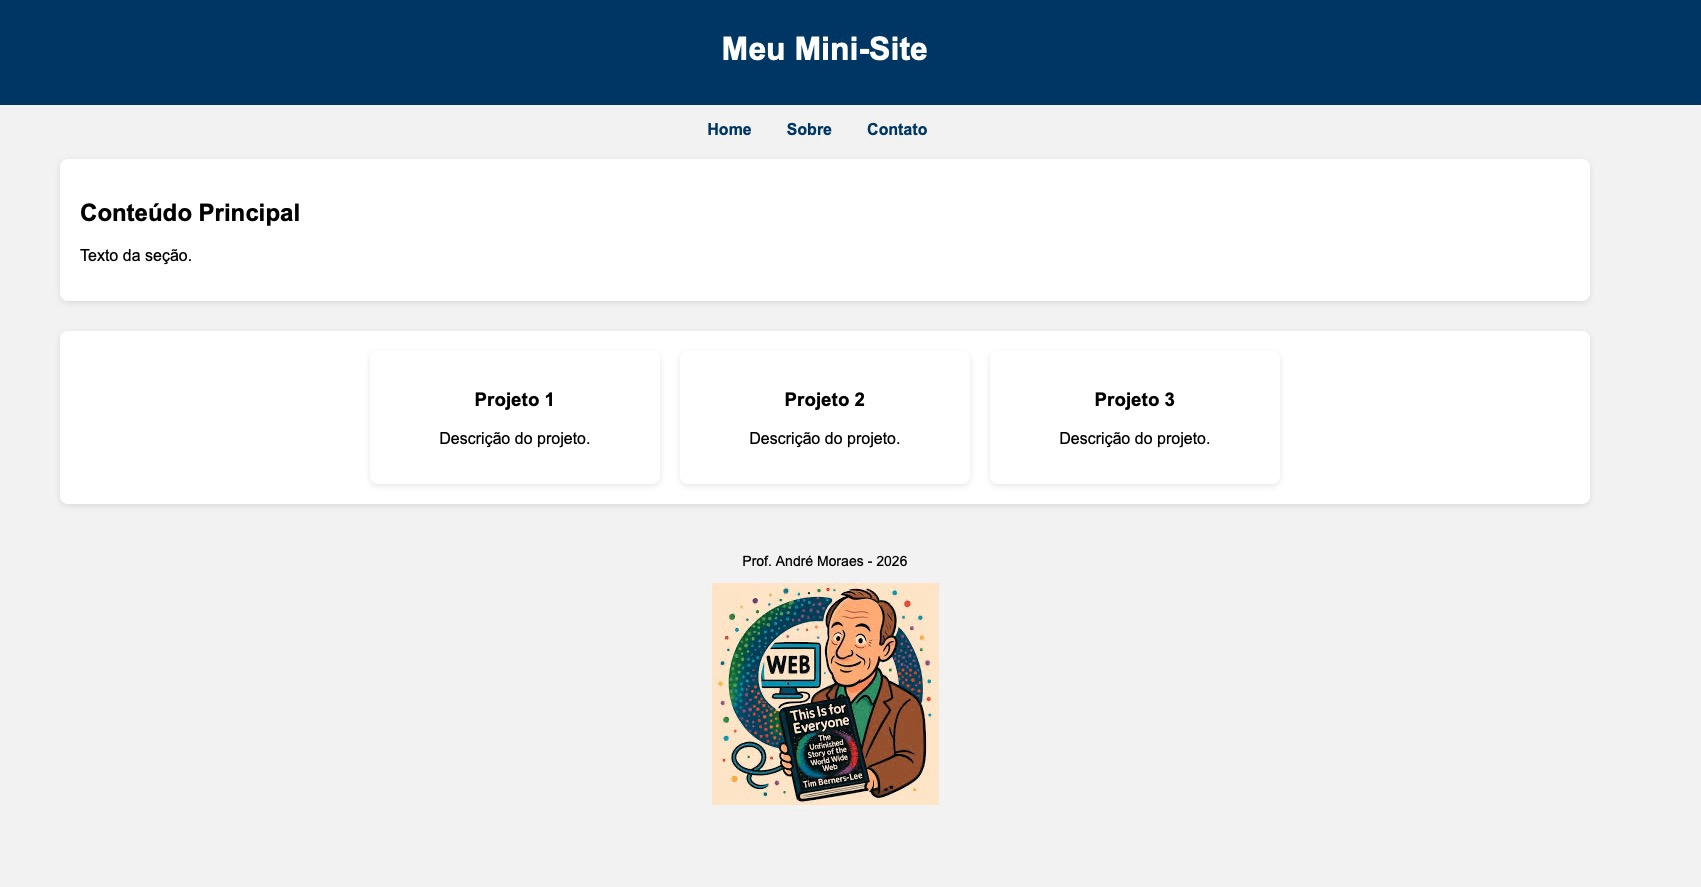
\includegraphics[width=0.9\textwidth]{figures/roteiro-04-layout-final.jpeg}}
    \caption{Layout final com cards organizados utilizando Flexbox.}
\end{figure}

% =====================================================
% VERSIONAMENTO
% =====================================================

\subsection{Versionamento}

\begin{boxCodigo}
\begin{verbatim}
git add .
git commit -m "Adiciona seção de cards com flexbox"
git push
\end{verbatim}
\end{boxCodigo}

% =====================================================
% CHECKLIST
% =====================================================

\subsection{Checklist Final}

\begin{boxAtividade}

\begin{itemize}
\item Projeto recuperado com Git;
\item Menu com Flexbox;
\item Seção de cards criada;
\item Cards estilizados;
\item Layout organizado;
\item Alterações versionadas.
\end{itemize}

\end{boxAtividade}

% =====================================================
% REPOSITÓRIO
% =====================================================

\subsection{Repositório Oficial da Unidade Curricular}

\begin{tcolorbox}[
colback=azulTitulo!5,
colframe=azulTitulo,
title=\textbf{Repositório Oficial da Disciplina}
]

\begin{center}
\qrcode[height=3cm]{https://github.com/chameoandre/uc-prog-internet-2026.git}
\end{center}

\begin{center}
\texttt{https://github.com/chameoandre/uc-prog-internet-2026.git}
\end{center}

\end{tcolorbox}


\newpage





% =====================================================
% ROTEIRO PRÁTICO 05
% =====================================================

\section{Roteiro Prático 05 — Responsividade e Evolução dos Cards}

% =====================================================
% OBJETIVOS
% =====================================================

\subsection{Objetivos da Aula}

\begin{boxObjetivos}
Ao final desta aula o estudante será capaz de:

\begin{itemize}
\item Evoluir o layout criado com Flexbox;
\item Trabalhar com imagens dentro dos cards;
\item Diferenciar quando substituir ou adicionar código CSS;
\item Aplicar responsividade com Media Queries;
\item Melhorar a organização visual do site.
\end{itemize}
\end{boxObjetivos}

% =====================================================
% INTRODUÇÃO
% =====================================================

\subsection{Introdução}

No roteiro anterior, criamos uma seção de cards utilizando Flexbox.

Agora, vamos evoluir esse layout com melhorias visuais e adaptação para diferentes tamanhos de tela.

Nesta aula, será importante compreender a diferença entre:

\begin{itemize}
\item \textbf{Substituir código existente} (quando corrigimos ou melhoramos algo);
\item \textbf{Adicionar código novo} (quando incluímos funcionalidades).
\end{itemize}

% =====================================================
% PREPARAÇÃO
% =====================================================

\subsection{Preparação do Ambiente}

Antes de iniciar a aula, é necessário garantir que o projeto esteja atualizado na sua máquina.

\subsubsection{Situação 1 — Projeto já existe no computador}

Se você já possui o projeto salvo na máquina, acesse a pasta do projeto e execute:

\begin{boxCodigo}
\begin{verbatim}
git pull
\end{verbatim}
\end{boxCodigo}

Isso irá atualizar o projeto com as versões mais recentes do GitHub.

\subsubsection{Situação 2 — Novo computador ou projeto não encontrado}

Se você está em outro computador ou não possui o projeto salvo, será necessário cloná-lo novamente:

\begin{boxCodigo}
\begin{verbatim}
git clone https://github.com/SEU-USUARIO/prog-internet-2026.git
\end{verbatim}
\end{boxCodigo}

Após isso, acesse a pasta do projeto:

\begin{boxCodigo}
\begin{verbatim}
cd prog-internet-2026
\end{verbatim}
\end{boxCodigo}

E entre na pasta do último roteiro:

\begin{boxCodigo}
\begin{verbatim}
cd roteiro-5
\end{verbatim}
\end{boxCodigo}

\subsubsection{Situação 3 — Dúvidas sobre o estado do projeto}

Caso você não tenha certeza se seu projeto está atualizado:

\begin{itemize}
\item Execute \texttt{git pull};
\item Verifique se os arquivos estão presentes;
\item Em caso de erro, consulte o professor.
\end{itemize}

\begin{boxDica}
\textbf{Importante:}

Nunca recrie o projeto manualmente.  
Sempre utilize o \texttt{git clone} para manter o histórico de versões.
\end{boxDica}


\newpage

% =====================================================
% PARTE 1 — IMAGENS NOS CARDS
% =====================================================

\subsection{Parte 1 — Adicionando Imagens}

\subsubsection{Atualize o HTML}

\begin{boxCodigo}
\begin{verbatim}
<div class="card">
    <img src="assets/img/projeto1.jpg" alt="Projeto 1">
    <h3>Projeto 1</h3>
    <p>Descrição do projeto.</p>
</div>
\end{verbatim}
\end{boxCodigo}

\begin{boxAtividade}[Atividade 1]

\begin{itemize}
\item Inserir imagens em todos os cards;
\item Garantir que as imagens estejam na pasta correta;
\item Testar o carregamento no navegador.
\end{itemize}

\end{boxAtividade}

% =====================================================
% PARTE 2 — AJUSTE DO CSS (SUBSTITUIÇÃO)
% =====================================================

\subsection{Parte 2 — Ajustando os Cards (Substituição)}

Agora vamos \textbf{substituir} parte do CSS existente para melhorar o comportamento dos cards.

\subsubsection{Substitua a classe \texttt{.cards}}

\begin{boxCodigo}
\begin{verbatim}
.cards{
    display: flex;
    gap: 20px;
    justify-content: center;
    text-align: center;
}
\end{verbatim}
\end{boxCodigo}

\subsubsection{Substitua a classe \texttt{.card}}

\begin{boxCodigo}
\begin{verbatim}
.card{
    display: flex;
    flex-direction: column;
    background-color: white;
    padding: 20px;
    width: 250px;
    border-radius: 8px;
    box-shadow: 0px 2px 6px rgba(0,0,0,0.1);
    text-align: center;
}
\end{verbatim}
\end{boxCodigo}

\begin{boxDica}
A propriedade \texttt{flex-direction} só funciona corretamente quando usamos \texttt{display: flex}.
\end{boxDica}

% =====================================================
% PARTE 3 — LIMPEZA DO MENU
% =====================================================

\subsection{Parte 3 — Ajustando o Menu}

Remova o trecho abaixo do seu CSS:

\begin{boxCodigo}
\begin{verbatim}
nav li {
    display: inline;
}
\end{verbatim}
\end{boxCodigo}

\begin{boxDica}
Quando utilizamos Flexbox, não precisamos utilizar \texttt{display: inline}.
\end{boxDica}

% =====================================================
% PARTE 4 — NOVOS ESTILOS (ADIÇÃO)
% =====================================================

\subsection{Parte 4 — Adicionando Novos Estilos}

Agora vamos \textbf{adicionar} novos estilos ao final do arquivo CSS.

\subsubsection{Imagens nos cards}

\begin{boxCodigo}
\begin{verbatim}
.card img {
    width: 100%;
    border-radius: 5px;
    margin-bottom: 10px;
}
\end{verbatim}
\end{boxCodigo}

\subsubsection{Efeito visual}

\begin{boxCodigo}
\begin{verbatim}
.card:hover {
    transform: translateY(-5px);
    box-shadow: 0px 4px 12px rgba(0,0,0,0.2);
    transition: all 0.3s ease;
}
\end{verbatim}
\end{boxCodigo}

% =====================================================
% PARTE 5 — RESPONSIVIDADE
% =====================================================

\subsection{Parte 5 — Responsividade}

Agora vamos tornar o layout adaptável para telas menores.

\begin{boxCodigo}
\begin{verbatim}
@media(max-width: 768px){
    .cards{
        flex-direction: column;
        align-items: center;
    }
}
\end{verbatim}
\end{boxCodigo}

\begin{boxAtividade}[Atividade 2]

\begin{itemize}
\item Redimensionar o navegador;
\item Verificar comportamento dos cards;
\item Testar em tela menor.
\end{itemize}

\end{boxAtividade}

% =====================================================
% RESULTADO FINAL
% =====================================================

\subsection{Resultado Final Esperado}

\begin{figure}[h!]
    \centering
    \fbox{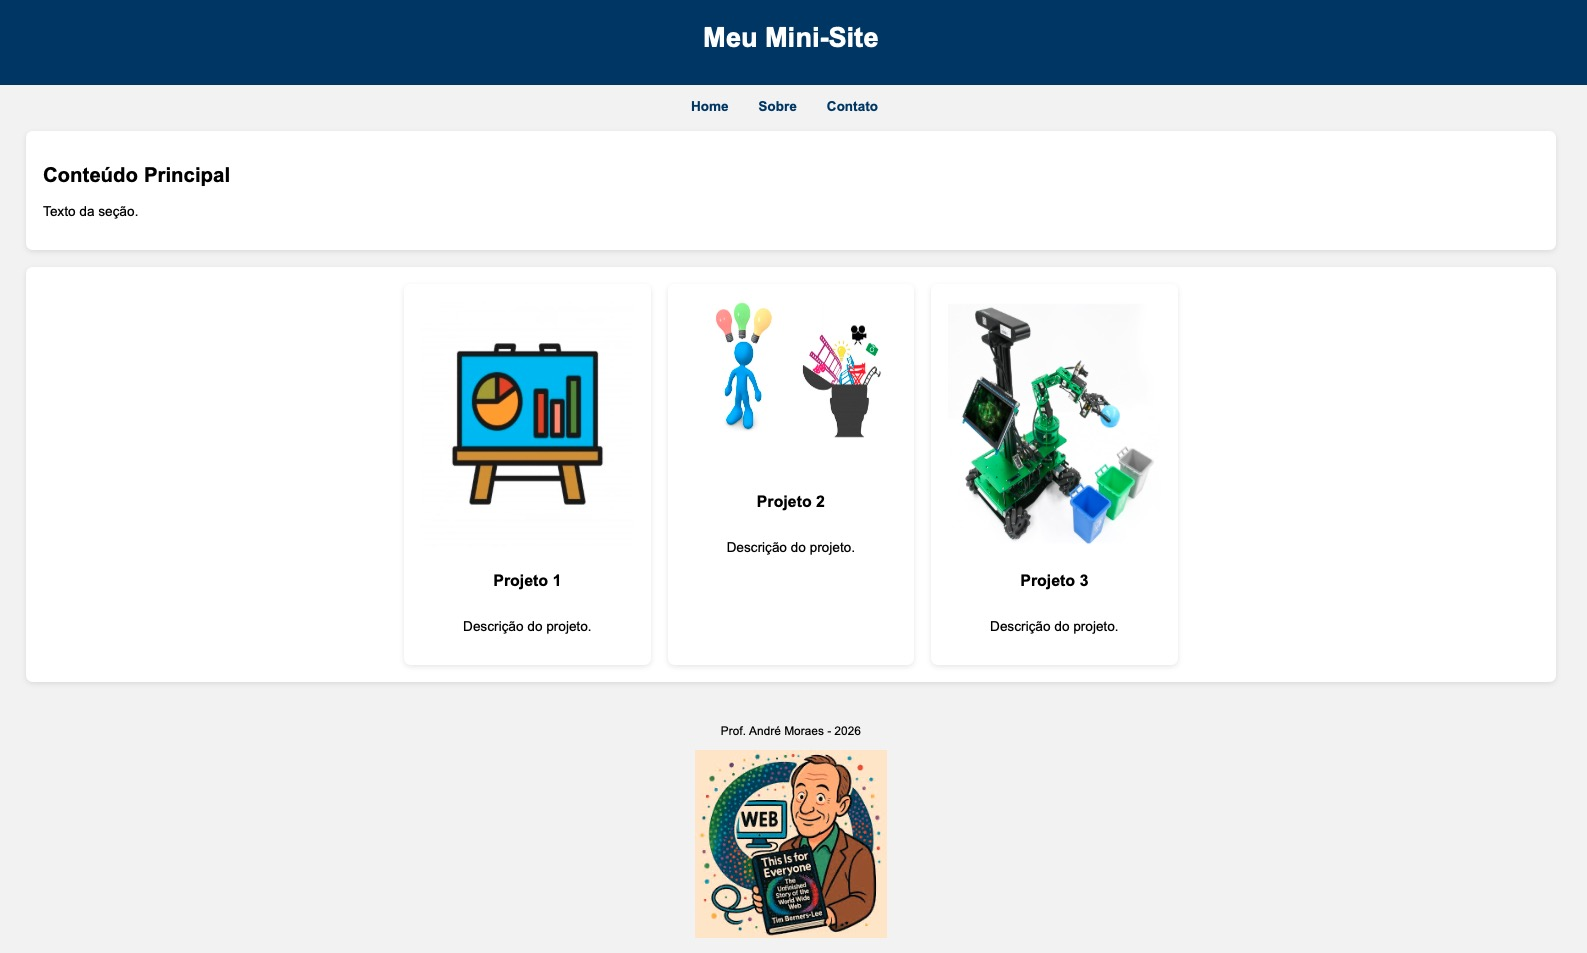
\includegraphics[width=0.9\textwidth]{figures/roteiro-5-checkpoint-1.jpg}}
    \caption{Cards com imagens e comportamento responsivo.}
\end{figure}



% =====================================================
% VERSIONAMENTO
% =====================================================

\subsection{Versionamento}

\begin{boxCodigo}
\begin{verbatim}
git add .
git commit -m "Melhoria visual e responsividade dos cards"
git push
\end{verbatim}
\end{boxCodigo}

% =====================================================
% CHECKLIST
% =====================================================

\subsection{Checklist Final}

\begin{boxAtividade}

\begin{itemize}
\item Cards com imagens;
\item CSS atualizado corretamente;
\item Código substituído onde necessário;
\item Novos estilos adicionados;
\item Responsividade funcionando;
\item Projeto versionado.
\end{itemize}

\end{boxAtividade}

% =====================================================
% DESAFIO EXTRA
% =====================================================

\subsection{Desafio Extra}

\begin{boxAtividade}

\begin{itemize}
\item Criar um quarto card;
\item Alterar cores dos cards;
\item Inserir botão nos cards;
\item Personalizar layout.
\end{itemize}

\end{boxAtividade}



% =====================================================
% RESUMO DE PROPRIEDADES CSS UTILIZADAS
% =====================================================

\subsection{Resumo das Propriedades CSS Utilizadas}

    A tabela abaixo apresenta as principais propriedades CSS utilizadas ao longo dos roteiros e suas funções dentro do site desenvolvido.
    
    \begin{boxTabela}
    \rowcolors{2}{cinzaTabela!20}{white}
    \begin{tabular}{|p{4cm}|p{5cm}|p{7cm}|}
    \hline
    \rowcolor{pretoTabela}
    \color{white}\textbf{Propriedade} &
    \color{white}\textbf{Onde foi usada} &
    \color{white}\textbf{Função} \\
    \hline
    
    display: flex & Menu e cards & Organiza elementos em linha de forma flexível \\
    \hline
    
    justify-content & Menu e cards & Alinha elementos horizontalmente \\
    \hline
    
    gap & Menu e cards & Define espaçamento entre elementos \\
    \hline
    
    flex-direction & Cards & Define a direção dos elementos (coluna nos cards) \\
    \hline
    
    width & Container e cards & Define largura dos elementos \\
    \hline
    
    margin & Container & Centraliza elementos na página \\
    \hline
    
    padding & Cards e sections & Define espaçamento interno \\
    \hline
    
    background-color & Header, section, cards & Define cor de fundo \\
    \hline
    
    color & Textos e links & Define cor do texto \\
    \hline
    
    border-radius & Cards e sections & Arredonda os cantos dos elementos \\
    \hline
    
    box-shadow & Cards e sections & Adiciona sombra para destacar elementos \\
    \hline
    
    text-align & Vários elementos & Alinha o texto \\
    \hline
    
    text-decoration & Links & Remove sublinhado dos links \\
    \hline
    
    font-weight & Links & Deixa o texto em negrito \\
    \hline
    
    hover & Links e cards & Aplica efeito visual ao passar o mouse \\
    \hline
    
    transform & Cards & Cria efeito de animação (movimento/escala) \\
    \hline
    
    @media & Layout geral & Permite responsividade para diferentes telas \\
    \hline

\end{tabular}
\end{boxTabela}



\begin{boxDica}
\textbf{Dica de estudo:}

Revise esta tabela antes das próximas aulas.  
Todas as propriedades aqui foram utilizadas no seu próprio projeto.
\end{boxDica}



% =====================================================
% REPOSITÓRIO
% =====================================================

\subsection{Repositório Oficial da Unidade Curricular}

\begin{tcolorbox}[
colback=azulTitulo!5,
colframe=azulTitulo,
title=\textbf{Repositório Oficial da Disciplina}
]

\begin{center}
\qrcode[height=3cm]{https://github.com/chameoandre/uc-prog-internet-2026/tree/main/roteiro-5/}
\end{center}

\begin{center}
\texttt{Configura o conteúdo do roteiro 5 online}
\end{center}

\end{tcolorbox}


\newpage




% =====================================================
% ROTEIRO PRÁTICO 06
% =====================================================
\section{Roteiro Prático 06 — Formulários e Estilização Avançada com HTML5 e CSS3}

% =====================================================
% OBJETIVOS
% =====================================================

\subsection{Objetivos da Aula}

\begin{boxObjetivos}
Ao final desta aula o estudante será capaz de:

\begin{itemize}
\item Criar formulários modernos com HTML5;
\item Aplicar validações automáticas;
\item Melhorar a experiência do usuário (UX);
\item Estilizar formulários com CSS3;
\item Compreender o funcionamento dos principais atributos utilizados.
\end{itemize}
\end{boxObjetivos}

% =====================================================
% INTRODUÇÃO
% =====================================================

\subsection{Introdução}

Nesta aula, iremos evoluir o formulário criado anteriormente, tornando-o mais completo e visualmente profissional.

Além disso, vamos entender melhor como funcionam os atributos de validação do HTML5 e como o CSS pode melhorar a interação com o usuário.

% =====================================================
% PARTE 1 — HTML
% =====================================================

\subsection{Parte 1 — Estrutura do Formulário}

Nesta etapa, vamos reorganizar o formulário, incluindo novos campos e melhorando a experiência do usuário.

\subsubsection{Atualize o HTML}

\begin{boxCodigo}
\begin{verbatim}
<form class="form-contato">

    <h2>Formulário de Contato</h2>

    <label for="nome">Nome:</label>
    <input type="text" id="nome" required minlength="3" placeholder="Digite seu nome">

    <label for="email">Email:</label>
    <input type="email" id="email" required placeholder="exemplo@email.com">

    <label for="telefone">Telefone:</label>
    <input type="tel" id="telefone" pattern="[0-9]{10,11}" placeholder="Somente números">

    <label for="assunto">Assunto:</label>
    <select id="assunto">
        <option value="">Selecione</option>
        <option value="duvida">Dúvida</option>
        <option value="sugestao">Sugestão</option>
        <option value="contato">Contato</option>
    </select>

    <label for="mensagem">Mensagem:</label>
    <textarea id="mensagem" rows="4" required></textarea>

    <button type="submit">Enviar</button>

</form>
\end{verbatim}
\end{boxCodigo}

\begin{boxDica}
O HTML5 já possui validações automáticas para vários tipos de campo.
\end{boxDica}

% =====================================================
% PARTE 2 — CSS BASE
% =====================================================

\subsection{Parte 2 — Estrutura Visual do Formulário}

Agora vamos estruturar o formulário visualmente.

\begin{boxCodigo}
\begin{verbatim}
form {
    display: flex;
    flex-direction: column;
    gap: 12px;
    background-color: white;
    padding: 20px;
    border-radius: 8px;
    box-shadow: 0px 2px 6px rgba(0,0,0,0.1);
    max-width: 500px;
    margin: 20px auto;
}
\end{verbatim}
\end{boxCodigo}

\subsection{Parte 3 — Estilização dos Campos}

Nesta etapa, melhoramos a aparência dos campos.

\begin{boxCodigo}
\begin{verbatim}
input, textarea, select {
    padding: 10px;
    border: 1px solid #ccc;
    border-radius: 5px;
    font-size: 14px;
}
\end{verbatim}
\end{boxCodigo}

% =====================================================
% PARTE 4 — INTERAÇÃO
% =====================================================

\subsection{Parte 4 — Interação com o Usuário}

Aqui adicionamos feedback visual ao usuário.

\begin{boxCodigo}
\begin{verbatim}
input:focus, textarea:focus, select:focus {
    outline: none;
    border-color: #003366;
    box-shadow: 0 0 5px rgba(0,51,102,0.3);
}
\end{verbatim}
\end{boxCodigo}

% =====================================================
% PARTE 5 — BOTÃO
% =====================================================

\subsection{Parte 5 — Botão Interativo}

\begin{boxCodigo}
\begin{verbatim}
button {
    background-color: #003366;
    color: white;
    padding: 12px;
    border: none;
    border-radius: 5px;
    cursor: pointer;
    transition: background-color 0.3s ease;
}

button:hover {
    background-color: #0055aa;
}
\end{verbatim}
\end{boxCodigo}

% =====================================================
% PARTE 6 — VALIDAÇÃO VISUAL
% =====================================================

\subsection{Parte 6 — Validação Visual}

Agora vamos mostrar ao usuário se o campo está correto ou não.

\begin{boxCodigo}
\begin{verbatim}
input:valid {
    border-color: green;
}

input:invalid {
    border-color: red;
}
\end{verbatim}
\end{boxCodigo}

% =====================================================
% PARTE 7 — RESPONSIVIDADE
% =====================================================

\subsection{Parte 7 — Responsividade}

\begin{boxCodigo}
\begin{verbatim}
@media(max-width: 768px){
    form {
        width: 90%;
    }
}
\end{verbatim}
\end{boxCodigo}

% =====================================================
% TABELA FINAL
% =====================================================

\subsection{Tabela de Referência — HTML5 e CSS Utilizados}

\begin{boxTabela}
\rowcolors{2}{cinzaTabela!20}{white}
\begin{tabular}{|p{4cm}|p{6cm}|p{6cm}|}
\hline
\rowcolor{pretoTabela}
\color{white}\textbf{Elemento} &
\color{white}\textbf{Exemplo} &
\color{white}\textbf{Função} \\
\hline

required & input required & Campo obrigatório \\
\hline

type="email" & input type="email" & Valida formato de email \\
\hline

minlength & minlength="3" & Define tamanho mínimo \\
\hline

pattern & pattern="[0-9]{10,11}" & Define padrão (regex) \\
\hline

placeholder & placeholder="Digite..." & Texto de ajuda \\
\hline

display:flex & display: flex & Layout flexível \\
\hline

gap & gap: 10px & Espaçamento entre elementos \\
\hline

:focus & input:focus & Estilo ao clicar \\
\hline

:valid & input:valid & Campo válido \\
\hline

:invalid & input:invalid & Campo inválido \\
\hline

transition & transition: 0.3s & Animação suave \\
\hline

@media & @media(max-width:768px) & Responsividade \\
\hline

\end{tabular}
\end{boxTabela}




% =====================================================
% DESAFIO
% =====================================================

\subsection{Desafio Extra}

\begin{boxAtividade}

\begin{itemize}
\item Validar telefone com JavaScript;
\item Exibir mensagem personalizada sem usar alert;
\item Limpar o formulário após envio;
\item Criar validação mais avançada.
\end{itemize}

\end{boxAtividade}

\newpage



% =====================================================
% REPOSITÓRIO
% =====================================================

\subsection{Repositório Oficial do Roteiro 6}

\begin{tcolorbox}[
colback=azulTitulo!5,
colframe=azulTitulo,
title=\textbf{Repositório Oficial do Roteiro 6}
]

\begin{center}
\qrcode[height=3cm]{https://github.com/chameoandre/uc-prog-internet-2026/tree/main/roteiro-6/}
\end{center}

\begin{center}
\texttt{Configura o conteúdo do roteiro 6 online}
\end{center}

\end{tcolorbox}



\newpage






% =====================================================
% ROTEIRO PRÁTICO 07
% =====================================================

\section{Roteiro Prático 07 — Manipulação da Árvore DOM}

\begin{boxObjetivos}
\begin{itemize}
    \item Dominar os métodos de seleção: \texttt{getElementById} e \texttt{querySelector};
    \item Manipular dinamicamente o conteúdo da página (\texttt{innerText}, \texttt{innerHTML});
    \item Alterar estilos CSS e gerenciar classes (\texttt{classList});
    \item Criar e remover elementos HTML via JavaScript (\texttt{createElement}, \texttt{appendChild}).
\end{itemize}
\end{boxObjetivos}

\subsection{O que é o DOM?}
O \textbf{DOM (Document Object Model)} é a representação em árvore dos elementos do seu HTML que o navegador cria para que o JavaScript possa interagir com eles.

\subsection{Sintaxe Moderna: A Metáfora da Seta (Arrow Functions)}

\begin{boxDica}
\textbf{O Atalho do Chef (=>)}

Imagine que escrever código é como pedir um prato em um restaurante. Na forma antiga (\texttt{function}), você tinha que preencher um formulário longo: ``Eu declaro que gostaria de uma função que recebe um pedido e faz tal coisa...''.

Com a \textbf{Arrow Function} (\texttt{=>}), você usa um atalho. O símbolo \texttt{=>} é uma seta que aponta diretamente do **evento** para a **ação**. É como dizer: ``Quando o botão for clicado \textbf{=>} mude a cor''. É mais rápido, limpo e moderno!
\end{boxDica}

\subsection{Parte 1 — Selecionando e Alterando Elementos}

\begin{boxAtividade}[A Intenção do Código]
Nesta primeira atividade, vamos ensinar o navegador a ``olhar'' para um título específico e trocar a roupa (cor) dele. O JavaScript vai localizar o ID único e aplicar o novo estilo instantaneamente.
\end{boxAtividade}

\begin{boxAtividade}[Atividade prática 1 — Seletores e Texto]
Crie um arquivo \texttt{dom-test.html} e implemente:


\begin{boxCodigo}
\begin{verbatim}
<h1 id="titulo">Olá Mundo!</h1>
<button onclick="mudarTexto()">Clique Aqui</button>

<script>
function mudarTexto() {
    const titulo = document.getElementById("titulo");
    titulo.innerText = "JavaScript funcionando!";
    titulo.style.color = "blue";
}
</script>
\end{verbatim}
\end{boxCodigo}
\end{boxAtividade}

\subsection{Parte 2 — Tabelas de Referência de Métodos}

\begin{boxAtividade}[Guia de Métodos de Seleção]
\begin{center}
\rowcolors{2}{blue!5}{white}
\begin{tabular}{|l|p{10cm}|}
\hline
\rowcolor{azulTitulo} \color{white} \textbf{Método} & \color{white} \textbf{Descrição} \\ \hline
\texttt{getElementById()} & Busca um elemento pelo seu ID único. \\ \hline
\texttt{querySelector()} & Busca o primeiro elemento que valide o seletor CSS (ex: .classe, \#id, tag). \\ \hline
\texttt{querySelectorAll()} & Busca uma lista de todos os elementos que validam o seletor. \\ \hline
\end{tabular}
\end{center}
\end{boxAtividade}

\subsection{Parte 3 — Criação Dinâmica de Elementos}

Este é um dos conceitos mais importantes: fazer o HTML ``aparecer'' na tela via código.

\begin{boxAtividade}[A Intenção do Código]
Vamos criar do zero novos elementos, como se estivéssemos montando peças de LEGO na tela. Em vez de escrever o HTML manualmente, o JavaScript vai fabricar uma nova \texttt{<li>} toda vez que você clicar no botão.
\end{boxAtividade}

\begin{boxAtividade}[Atividade prática 2 — A Fábrica de Elementos]
Vamos criar uma lista onde cada clique no botão adiciona um novo item:

\begin{boxCodigo}
\begin{verbatim}
<ul id="minhaLista"></ul>
<button id="add">Adicionar Item</button>

<script>
const lista = document.getElementById("minhaLista");
const botao = document.getElementById("add");

botao.addEventListener("click", () => {
    // 1. Criar o elemento
    const novoItem = document.createElement("li");
    
    // 2. Dar conteúdo ao elemento
    novoItem.innerText = "Novo Item na Lista";
    
    // 3. Adicionar na página
    lista.appendChild(novoItem);
});
</script>
\end{verbatim}
\end{boxCodigo}
\end{boxAtividade}

\subsection{Parte 4 — Praticando com Estados e Atributos}

\begin{boxAtividade}[A Intenção do Código]
Agora vamos lidar com números e imagens. No primeiro exemplo, o JavaScript vai guardar um valor na memória (uma variável) e aumentá-lo a cada clique. No segundo, vamos manipular o atributo \texttt{src} para trocar uma imagem por outra, simulando um interruptor.
\end{boxAtividade}

\begin{boxAtividade}[Atividade prática 3 — O Contador de Cliques]
Crie um contador simples:

\begin{boxCodigo}
\begin{verbatim}
<h2 id="contador">0</h2>
<button id="btnSoma">Contar +1</button>

<script>
let valor = 0;
const display = document.getElementById("contador");

document.getElementById("btnSoma").addEventListener("click", () => {
    valor++;
    display.innerText = valor;
});
</script>
\end{verbatim}
\end{boxCodigo}
\end{boxAtividade}

\begin{boxAtividade}[Atividade prática 4 — Luz Acesa, Luz Apagada]
Troque a imagem dinamicamente (use links de imagens de lâmpadas ou placeholders):

\begin{boxCodigo}
\begin{verbatim}
<img id="lampada" src="off.png" style="width:100px">
<button id="btnInterruptor">Ligar/Desligar</button>

<script>
const img = document.getElementById("lampada");
let acesa = false;

document.getElementById("btnInterruptor").addEventListener("click", () => {
    acesa = !acesa;
    img.src = acesa ? "on.png" : "off.png";
});
</script>
\end{verbatim}
\end{boxCodigo}
\end{boxAtividade}

\subsection{Laboratório de Mini-Jogos Lúdicos}

\begin{boxAtividade}[A Intenção do Código]
Para consolidar o aprendizado, vamos transformar o código em jogo! Nestes desafios, o JavaScript deixa de ser apenas uma ferramenta de formulário e passa a gerenciar estados de jogo, aleatoriedade e reações rápidas ao mouse.
\end{boxAtividade}

\begin{boxAtividade}[Atividade prática 5 — Jogo de Adivinhação]
\textbf{Conceito:} O computador escolhe um número e você tenta adivinhar. O JS compara os valores e te dá dicas.

\begin{boxCodigo}
\begin{verbatim}
<input type="number" id="palpite" placeholder="0 a 10">
<button id="btnChutar">Chutar!</button>
<p id="feedback"></p>

<script>
const segredo = Math.floor(Math.random() * 11);
const campo = document.getElementById("palpite");
const texto = document.getElementById("feedback");

document.getElementById("btnChutar").addEventListener("click", () => {
    const chute = Number(campo.value);
    if (chute === segredo) {
        texto.innerText = "🎉 Parabéns! Você acertou!";
        texto.style.color = "green";
    } else {
        texto.innerText = chute > segredo ? "Muito alto!" : "Muito baixo!";
        texto.style.color = "red";
    }
});
</script>
\end{verbatim}
\end{boxCodigo}
\end{boxAtividade}

\begin{boxAtividade}[Atividade prática 6 — O Botão Fugitivo]
\textbf{Conceito:} Um botão que foge do mouse! Vamos aprender a mudar a posição absoluta do elemento e contar quantas vezes você falhou.

\begin{boxCodigo}
\begin{verbatim}
<p>Erros: <span id="contadorErros">0</span></p>
<button id="fugitivo" style="position: absolute; left: 50%; top: 50%;">
    Pegue-me!
</button>

<script>
const btn = document.getElementById("fugitivo");
const placar = document.getElementById("contadorErros");
let erros = 0;

btn.addEventListener("mouseover", () => {
    erros++;
    placar.innerText = erros;
    
    // Mudar posição aleatoriamente
    const x = Math.random() * (window.innerWidth - 100);
    const y = Math.random() * (window.innerHeight - 50);
    
    btn.style.left = `${x}px`;
    btn.style.top = `${y}px`;
});

btn.addEventListener("click", () => alert("🎯 Você me pegou!"));
</script>
\end{verbatim}
\end{boxCodigo}
\end{boxAtividade}

\begin{boxAtividade}[Atividade prática 7 — Jokenpô (Emoji Edition)]
\textbf{Conceito:} Pedra, Papel e Tesoura. O JavaScript decide o sorteio do computador e compara com a sua escolha.

\begin{boxCodigo}
\begin{verbatim}
<button onclick="jogar('🪨')">🪨</button>
<button onclick="jogar('📄')">📄</button>
<button onclick="jogar('✂️')">✂️</button>
<h3 id="resultadoJogo">Escolha um!</h3>

<script>
const opcoes = ['🪨', '📄', '✂️'];

function jogar(player) {
    const pc = opcoes[Math.floor(Math.random() * 3)];
    const res = document.getElementById("resultadoJogo");
    
    if (player === pc) {
        res.innerText = `Empate! Ambos escolheram ${pc}`;
    } else if (
        (player === '🪨' && pc === '✂️') ||
        (player === '📄' && pc === '🪨') ||
        (player === '✂️' && pc === '📄')
    ) {
        res.innerText = `Você Ganhou! ${player} vence ${pc}`;
    } else {
        res.innerText = `Você Perdeu! ${pc} vence ${player}`;
    }
}
</script>
\end{verbatim}
\end{boxCodigo}
\end{boxAtividade}

\newpage

\section{Roteiro Prático 08 — Requisições Assíncronas e Fetch API}

\begin{boxObjetivos}
\begin{itemize}
    \item Compreender o formato de dados JSON;
    \item Utilizar a Fetch API para buscar dados externos;
    \item Integrar o consumo de APIs com a manipulação do DOM.
\end{itemize}
\end{boxObjetivos}

\subsection{Entendendo o JSON}
JSON é o formato padrão de troca de mensagens na web moderna. Ele funciona como um objeto JavaScript formatado como texto.

\subsection{A Metáfora da Esteira de Produção (Fetch Chain)}

\begin{boxDica}
\textbf{A Esteira de Pedidos}

Imagine uma esteira de produção em uma lanchonete:
\begin{enumerate}
    \item \texttt{fetch} [O Pedido] **=>** Você faz o pedido no balcão (internet).
    \item \texttt{json()} [A Cozinha] **=>** O cozinheiro recebe o pedido bruto e o transforma em um prato pronto para comer (objeto JS).
    \item \texttt{dados} [O Garçom] **=>** Agora você pode pegar o prato e colocar na mesa (mostrar na tela).
\end{enumerate}
O encadeamento de \texttt{.then() => ...} é o movimento da esteira passando o pedido de uma mão para a outra.
\end{boxDica}

\subsection{Exploração Prática — O Projeto ViaCEP}

\begin{boxAtividade}[A Intenção do Código]
O fluxo aqui é completo: o usuário digita um CEP **=>** Nós perguntamos aos correios via internet **=>** Eles nos devolvem um pacote (JSON) **=>** Nós abrimos esse pacote e usamos o DOM para mostrar o endereço na tela sem recarregar a página.
\end{boxAtividade}

\begin{boxAtividade}[Atividade prática 3 — Integração Completa (Fetch + DOM)]
Integre a busca de CEP no seu projeto:

\begin{boxCodigo}
\begin{verbatim}
const cep = document.getElementById("cep").value;

fetch(`https://viacep.com.br/ws/${cep}/json/`)
    .then(response => response.json())
    .then(dados => {
        if (dados.erro) {
            document.getElementById("resultado").innerText = "Erro!";
        } else {
            document.getElementById("resultado").innerText = 
               `${dados.logradouro}, ${dados.localidade}`;
        }
    });
\end{verbatim}
\end{boxCodigo}
\end{boxAtividade}

\begin{boxAtividade}[Tabela de Referência — Comandos de Rede]
\begin{center}
\rowcolors{2}{blue!5}{white}
\begin{tabular}{|l|p{10cm}|}
\hline
\rowcolor{azulTitulo} \color{white} \textbf{Comando} & \color{white} \textbf{O que faz?} \\ \hline
\texttt{fetch(url)} & Inicia a requisição para o servidor. \\ \hline
\texttt{.then()} & Aguarda a promessa ser resolvida para executar a ação. \\ \hline
\texttt{response.json()} & Converte o pacote de texto recebido em objeto JS. \\ \hline
\end{tabular}
\end{center}
\end{boxAtividade}

\end{document}
